\section{Material und Methoden} % (fold)
    \label{sec:material_und_methoden}
    Es werden drei Versuchsmedien erstellt, um das Wachstum differenziert betrachten zu können. Dabei wird eines mit normalem Leitungswasser gewässert, eines mit Salzwasser und eines mit angesäuertem Wasser. Der Salzgehalt von Zweitem soll bei $0,1 \frac{mol}{l}$ liegen. Dementsprechend werden dazu 5,85g NaCl in 100ml Leitungswasser gelöst und anschließend zu einem Liter aufgefüllt (Werte siehe \autoref{equ:nacl}).
    \begin{equation}\label{equ:nacl}
        \begin{split}  
        m(NaCl) &= 0,1\frac{mol}{l} * V(H_2O) * M(NaCl)\\
        &= 0,1\frac{mol}{l} * 1l * 58,5\frac{g}{mol}\\
        & = 5,85g
        \end{split}
    \end{equation}
    Das saure Medium soll einen pH-Wert von 5 haben. Zur Verfügung steht Essigessenz mit dem pH-Wert 2,65, sodass von dieser 4,5ml zu einem Liter aufgefüllt werden (siehe \autoref{equ:essig}).
    \begin{equation}
        \label{equ:essig}
        \begin{split}
            pH(Essig) & = 2,65 \\
            \Rightarrow c(H^+)_{alt} &=10^{-2,65}\\
            c(H^+)_{neu}&=10^{-5}\ \ \ \ =10^{-2,65} * x\\
            x&=\frac{10^{-5}}{10^{-2,65}} =0,0045
        \end{split}
    \end{equation}
    \begin{table}[h]
        \caption{Materialien}
        \label{tab:materials}
        \csvreader[tabular=rrrr,
            respect percent,
            table head=\toprule\centerIt{\textbf{Material}} & \centerIt{\textbf{Menge}} & \centerIt{\textbf{Zweck}} & \centerIt{\textbf{Zusatzinfo}}\\\midrule,
            /csv/separator=semicolon,
            head to column names,
            late after last line=\\\bottomrule]
            {../Materials.csv}{}
            {\Material&\Menge&\Zweck&\Zusatzinfo}
    \end{table}
    \subsection{Durchführung} % (fold)
        \label{sub:durchführung}
    
    % subsection durchführung (end)
% section material_und_methoden (end)

\newpage
\section{Ergebnisse} % (fold)
    \label{sec:ergebnisse}
    Text

    \begin{table}[h]
        \centering
        \caption{t-Test-Ergebnisse}
        \label{tab:t_test}
        \csvreader[tabular=rrr,
          table head=\toprule\centerIt{\textbf{Nullhypothese}} & \centerIt{\textbf{Sauer}} & \centerIt{\textbf{Salzig}}\\\midrule,
          /csv/separator=semicolon,
          head to column names,
          late after line=\\,
          late after last line=\\\bottomrule
          ]%
          {../Results/t_tests.csv}{H0=\H}%
        {\H & \pH & \NaCl}
    \end{table}
    Wie in \autoref{tab:t_test} zu sehen ist, \dots Die Quantile sind bla und bla\ \cite[vgl.][]{web:t-values} und bla\ \cite[vgl.][]{web:Gartenratgeber}\\

    \begin{figure}[ht]
        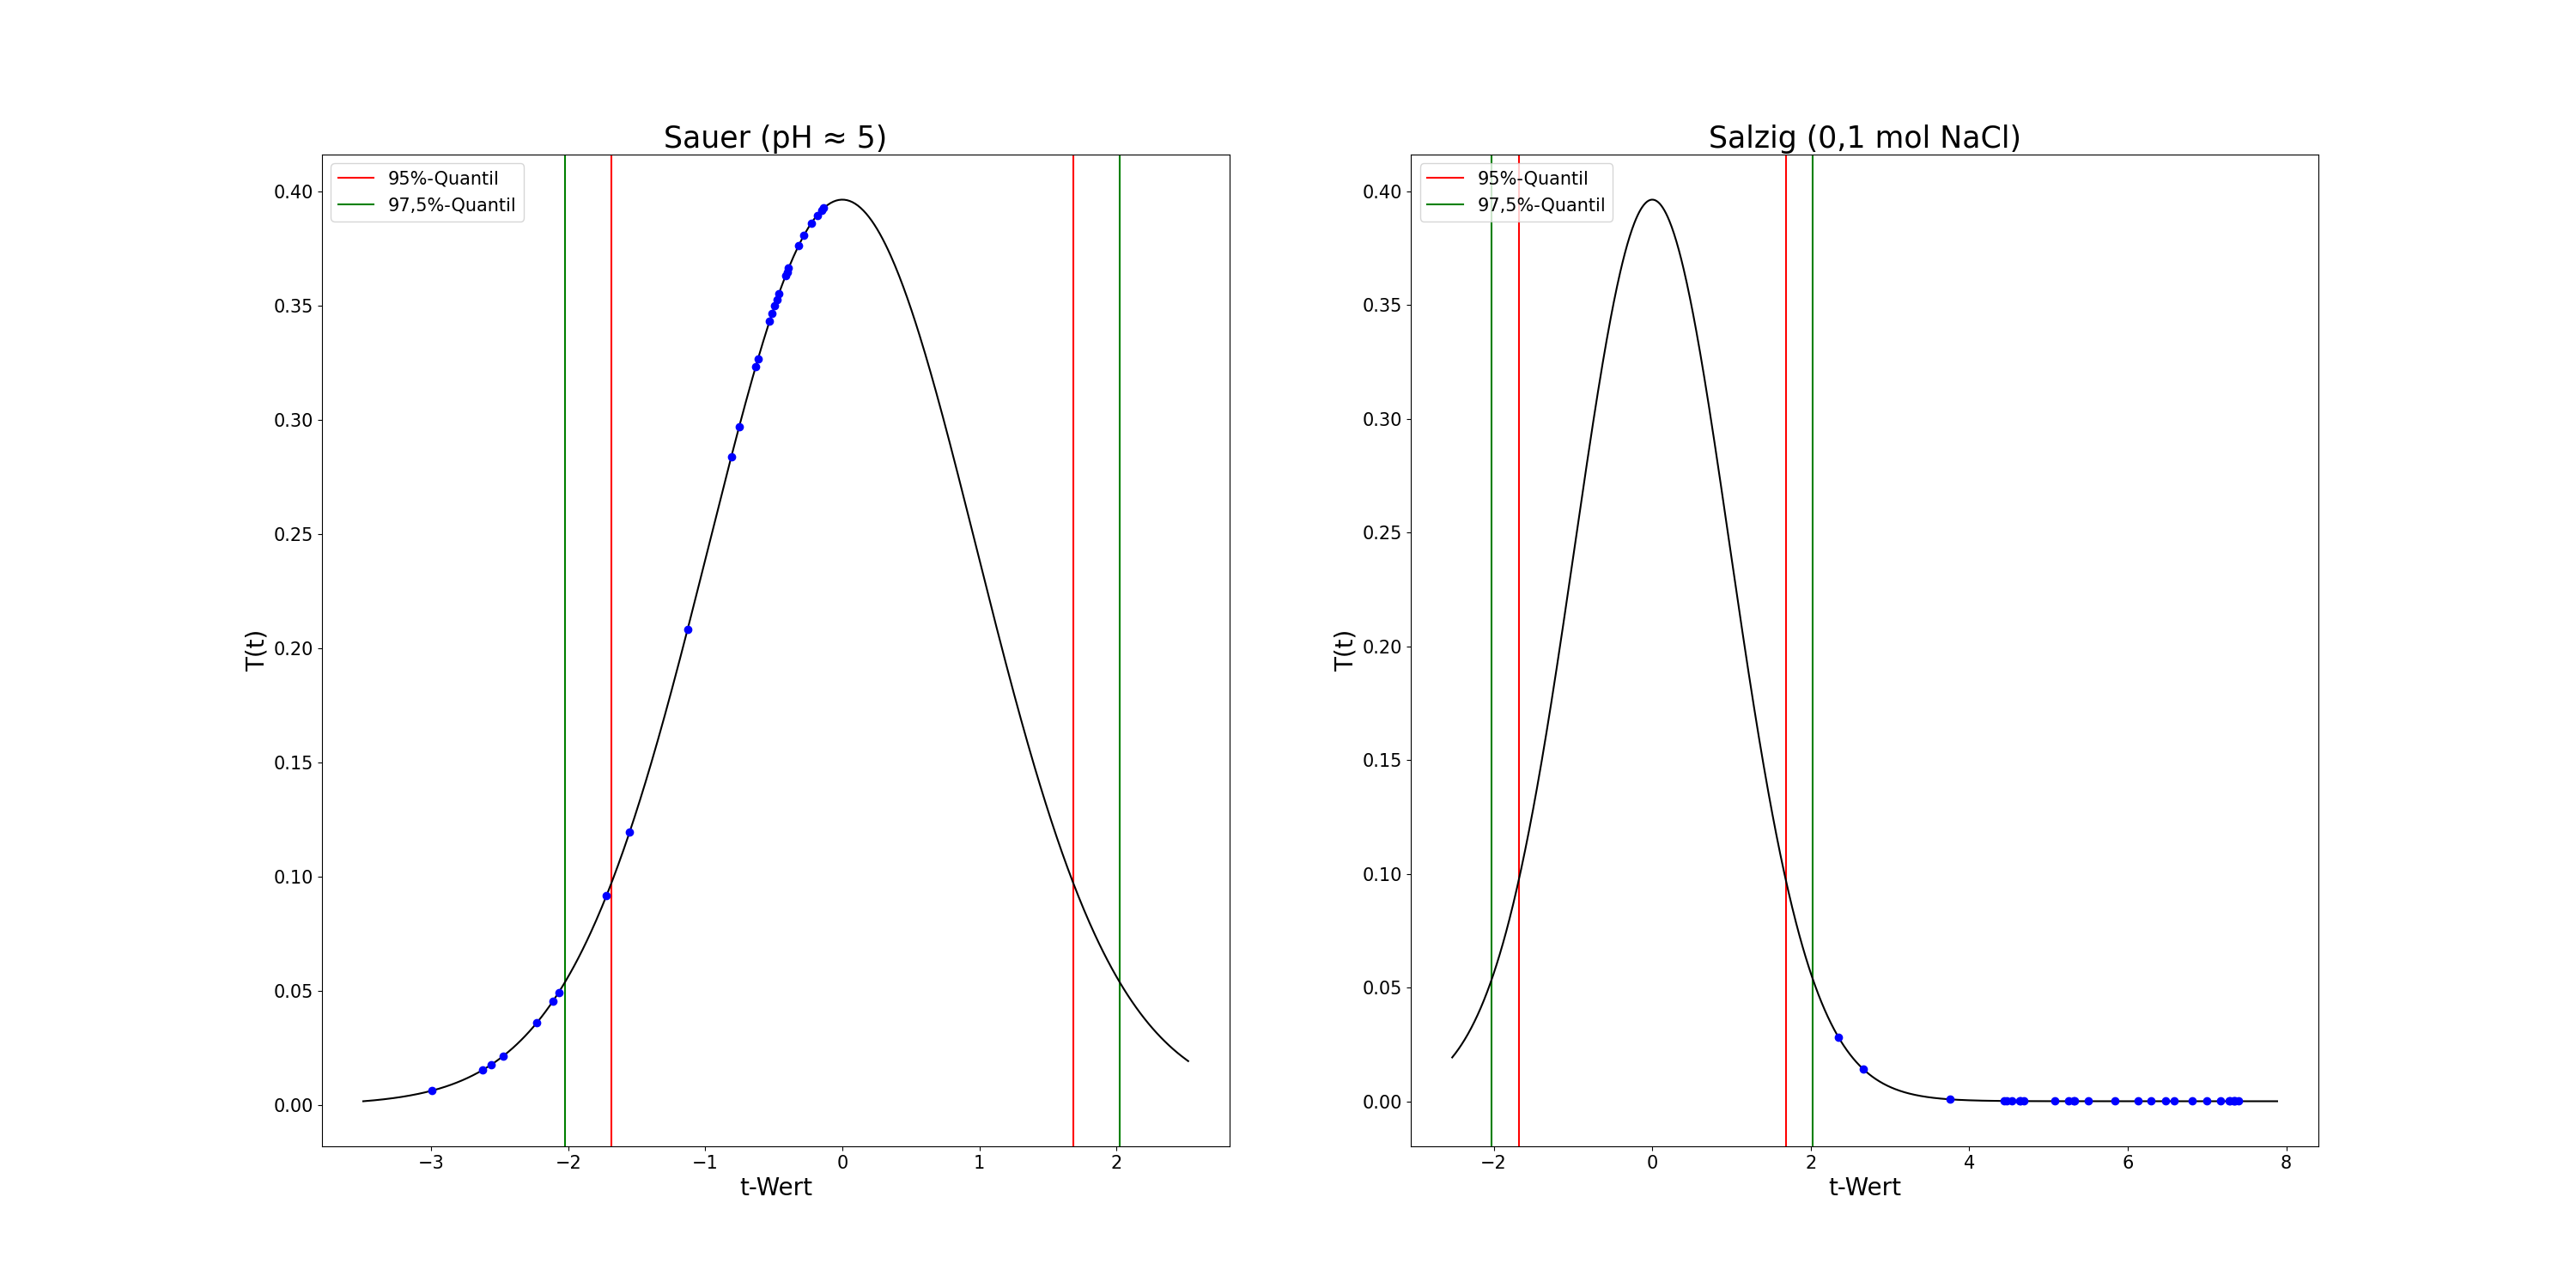
\includegraphics[width=1\textwidth]{t_tests.png}
        \caption{t-Tests}
        \label{fig:t_tests}
    \end{figure}
    asdasdasdasdasdasd\newpage

    \begin{figure}[ht]
        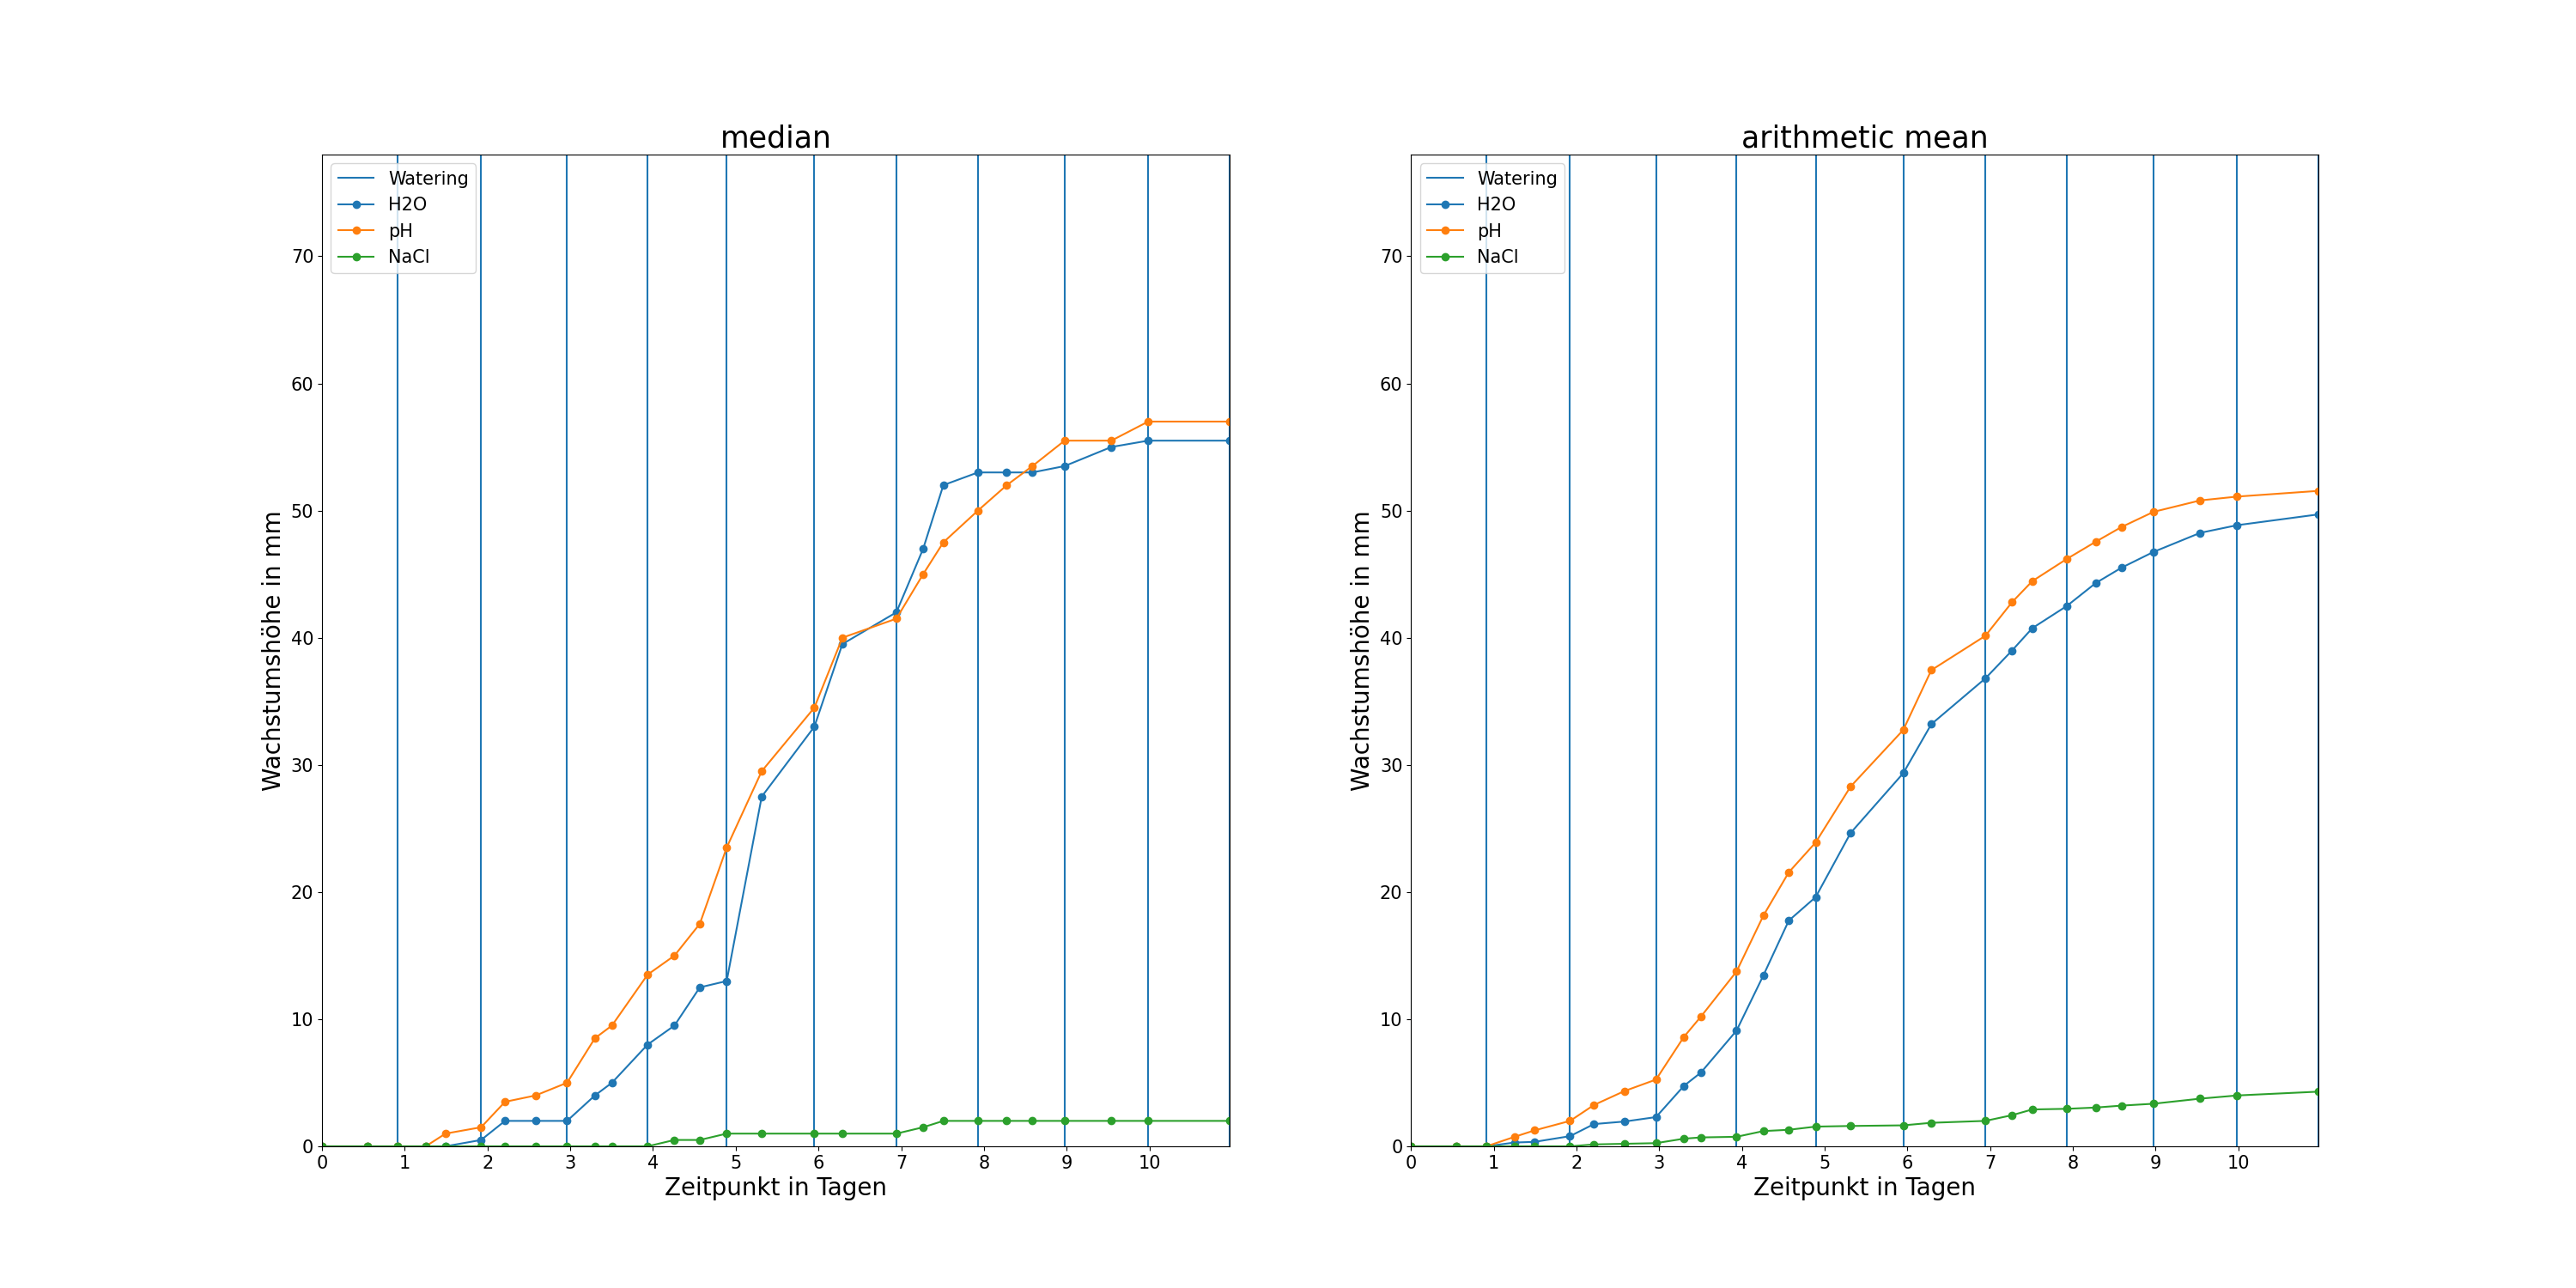
\includegraphics[width=1\textwidth]{ScatterPlot.png}
        \caption{Messwerte}
        \label{fig:scat_plot}
    \end{figure}\newpage

    \begin{figure}[ht]
        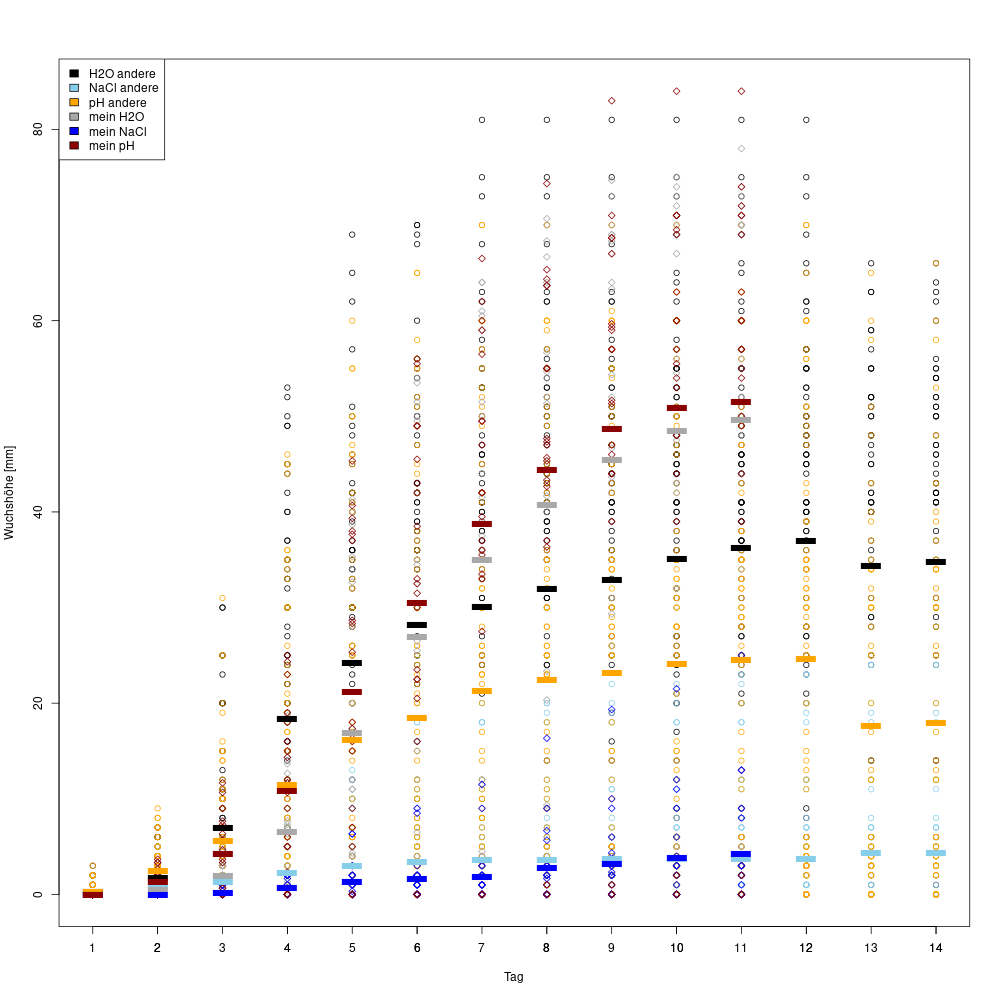
\includegraphics[width=1\textwidth]{scatterplot_my_vs_others.png}
        \caption{Wertevergleich mit anderen Durchführungen}
        \label{fig:scat_plot_cmp}
    \end{figure}
% section ergebnisse (end)
